\documentclass{article}

\usepackage{graphicx}
\usepackage{multicol}
\usepackage{fullpage}
\usepackage{floatflt}
\usepackage{xspace}

\def\degC{$^{\circ}$C }
\def\degf{$^{\circ}$F }
\def\vol #1 {{\bf #1}, $\;\;$}
\def\refer{\par\noindent\hangindent\parindent\hangafter1}


\title{Herzmann Family Christmas Letter 2014}
\author{Daryl Herzmann${}^1$, Elizabeth Herzmann${}^1$, Margaret 
Herzmann${}^2$, AND Robert Herzmann${}^3$ \\
\it{${}^1$ Caretakers},
\it{${}^2$ Senior Child},
\it{${}^3$ Precious Baby}} 
\date{23 December 2014}

\makeatletter
\newenvironment{tablehere}
  {\def\@captype{table}}
  {}

\newenvironment{figurehere}
  {\def\@captype{figure}}
  {}
\makeatother

\newcommand{\Line}[0]{%
  \rule{0cm}{0cm}\\\hrule\rule{0cm}{0cm}%
}

\addtolength{\textheight}{1.5in}

\begin{document}
\maketitle

\begin{abstract}
This article summarizes the year's worth of activities for the Herzmann
Family.  2014 was another successful year of family expansion, 
supporting the economy through various expenditures, and propitiation of 
Uncle Sam via tax remittance.  \emph{Author's Note: The submission of this 
dossier was delayed this year due to sleep deprivation associated with the 
newest arrival.}

\end{abstract}

\Line

\begin{multicols}{2}

\section{Introduction} 

Last year's Christmas Letter (Herzmann et al 2013) was well received and 
there was additional demand for a second printing.  While the Impact 
Factor was rather low (read zero), it was decided to again offer this 
summary.  Our family's size has never been larger and the subsequent 
increase in noise level has been more than proportional.  Our family now 
constitutes four humans (Daryl "Daryl" (36), Elizabeth "Liz" (30), 
Margaret "Miss Maggie" (1), and Robert "Rob-Rob" (0)) and one cat (Snoopy 
(6)).

\subsection{Housing}

Our family continues to make our residence in the plush suburb of Des 
Moines known as Ankeny.  We will have new neighbors soon!  These new 
neighbors happen to be Liz's maternal and paternal relatives (read Daryl's 
in-laws), who have moved here from Lincoln, NE.  
They are not exactly next door, but we can see their house from 
our kitchen window!  This is an exciting time for the children to have 
their grandparents so close and an exciting time for the parents to have 
on-demand babysitting available.

\subsection{Conveyances}

Last year's letter loathed the lack of a mini-van for parlaying our 
growing family.  No direct action was taken on this issue and given the 
news found in Section 1.1, we now have access to a minivan as well!  Thank 
you Liz's parents for letting us borrow their van!

\subsection{Employment}
Daryl remains employed with Iowa State University and continues to work on 
his weather data collection stuff.  When folks ask him for good weather, 
he notes that he works in sales and not production.  His employment is on 
an annual basis and contingent on proposals getting funded.  If you are a 
funding agency reading this letter, please considering funding my research!

Liz continues her work at Johnston Middle School with 8th and 9th graders. 
The Science Olympiad program, which Liz coaches, continues to flourish. 
Liz and her co-coach have expanded the program to the High school, which 
now supports about 45 additional students.  They prepare after school 
daily for the State competition in April.  Liz will again mentor a student 
teacher in the Spring.  Liz enjoys mommy - Maggie time on Saturday 
mornings with story time at the local library and summer swim lessons.

\begin{figurehere}
 \centering   
 \resizebox{.95\columnwidth}{!}{\includegraphics[angle=0]{plots/two.ps}}
 \caption{Liz and the dependants prior to the first day of Fall 2014 
school.}
\end{figurehere}

Miss Maggie has not found employment at this time.  She seems to get shy 
around new people, so that makes getting a service type job difficult.  

Mr Robert is unemployed as well, so only half of our house works for a 
living which matches national demographics.

\section{Mr Robert}

Liz gave birth to our second child on 15 June 2014 in the early morning 
hours.  According to Daryl, this birth was even easier than the previous 
one (even without the usage of pain medications).  
Against Daryl's advice, Liz nearly gave birth while driving to the 
hospital.  She did kindly wait for Daryl to park the car prior to Robert's 
arrival a few minutes later at 2:53 AM.  Miss Maggie was not entirely sure 
of what to make of this new arrival. She did immediately bop him over the 
head to verify his existence.  She now refers to him as "Rob-Rob", which 
will probably be the nicest name she will ever use about him.  

Mr Robert is a happy baby and makes very expressive facial gestures.  The 
daycare has determined that his laugh sounds like Dr Sheldon Cooper of 
television's Big Bang Theory.  Mr Robert is desperate to start crawling
and walking; he has lots of ambition to be on the move.

\begin{tablehere}
 \begin{center}
  \begin{tabular}{|c|l|l|}
   \multicolumn{1}{c}{Child} &
   \multicolumn{1}{l}{Metric} &
   \multicolumn{1}{l}{Percentile} \\ \hline \hline
   Margaret & Weight: 23 9oz & 63 \\
   On: 14 Jul & Height: 33" & 86 \\
    & Head Size: 19" & 93 \\
   Robert & Weight: 18 12oz & 73 \\
   On: 15 Dec & Height: 27$\frac{3}{4}$" & 91 \\
    & Head Size: 17$\frac{3}{4}$" & 92 \\
\hline
  \end{tabular}
 \end{center}
 \caption{Family physical metrics. Mother's statistics were redacted.}
 \label{table:metrics}
\end{tablehere}

\begin{figurehere}
 \centering   
 \resizebox{.95\columnwidth}{!}{\includegraphics[angle=0]{plots/one.ps}}
 \caption{Daryl teaching the children how to drive tractor (pronounced tra-tich by Miss Maggie)
on Grandma Barb's farm.}
\end{figurehere}

\section{Miss Maggie}

Miss Maggie will celebrate her second birthday in January and will enjoy 
being the center of attention again.  She picks up on new things each day 
and is slowly learning the English alphabet by watching Wheel of Fortune
 (Sajak and White 2014).  For this Christmas, she got 
her first big girl bed in exchange for retiring her pacifier (an 
arrangement she did not offer).  She is a wonderful helper and likes to remove items
from their storage and then put them back in random order.  She also is
constantly scanning the skies for ducks and geese.

\begin{figurehere}
 \centering   
 \resizebox{.95\columnwidth}{!}{\includegraphics[angle=0]{plots/size.ps}}
 \caption{Actual and modeled family size.}
\end{figurehere}

\section{Summary}

Our family continues to grow in size and love. Figure 3 details the growth and
extrapolated forecast of size.  For the first Christmas in
the past three years, Liz is not pregnant (at least to the author's knowledge).  
We may not be able to report
an increase in family size for next year's article unless we acquire another
feline.

\bigskip
  \emph{Acknowledgments} Our family wishes to thank you for the generous 
support, prayers, cards, gifts, and visits you have provided us in the past
year. With your continued support, this letter will be produced again
next year. Please note that the format chosen for this correspondence was
completely Daryl's idea and execution. Full \LaTeX\xspace source can be found on 
Daryl's github page.

\section{References}

\refer Github, 2014: https://github.com/akrherz/me , visited 23 Dec 2014.
\refer Herzmann, Daryl E., et al. Herzmann Family Christmas Letter 2013. 
\refer Sajak, Pat L. and Vanna M. White. America's Game. Wheel Watcher number 
available upon request. 

\end{multicols}

\end{document}

